\documentclass{article}
\usepackage{fancyhdr} % Required for custom headers
\usepackage{lastpage} % Required to determine the last page for the footer
\usepackage{extramarks} % Required for headers and footers
\usepackage[usenames,dvipsnames]{color} % Required for custom colors
\usepackage{graphicx} % Required to insert images
\usepackage{listings} % Required for insertion of code
\usepackage{courier} % Required for the courier font
\usepackage{caption}
\usepackage{subcaption}
\usepackage{amsmath}
\usepackage{amsfonts}
\usepackage{amssymb}
\usepackage{epstopdf}
\usepackage{placeins}
\usepackage{color} 
\usepackage{fancyvrb} 
\usepackage{setspace}
\usepackage[numbered]{bookmark}
\usepackage{tikz}
\usepackage{pgfplots}
\usepackage[absolute,overlay]{textpos}
\usetikzlibrary{calc}
\usetikzlibrary{pgfplots.fillbetween, backgrounds}
\usetikzlibrary{positioning}
\usetikzlibrary{arrows}
\usetikzlibrary{pgfplots.groupplots}
\usetikzlibrary{arrows.meta}
\usetikzlibrary{plotmarks}

\usepgfplotslibrary{groupplots}
\pgfplotsset{compat=newest} 
%\pgfplotsset{plot coordinates/math parser=false}
\DeclareGraphicsExtensions{.pdf,.png,.jpg}
\graphicspath{{figs/}}


\DeclareMathOperator{\E}{\mathbb{E}}
\newcommand{\Conv}{\mathop{\scalebox{1.5}{\raisebox{-0.2ex}{$\ast$}}}}%


% rect results in 1 if a < x < b, and 0 otherwise
\pgfmathdeclarefunction{rect}{3}{%
	\pgfmathparse{(and(#1 >= #2, #1 <= #3) * 1.0}%
}

\pgfplotsset{
	dirac/.style={
		mark=triangle*,
		mark options={scale=2},
		ycomb,
		scatter,
		visualization depends on={y/abs(y)-1 \as \sign},
		scatter/@pre marker code/.code={\scope[rotate=90*\sign,yshift=-2pt]}
	}
}

% Margins
\topmargin=-0.45in
\evensidemargin=0in
\oddsidemargin=0in
\textwidth=6.5in
\textheight=9.0in
\headsep=0.25in

\linespread{1.2} % Line spacing

% Set up the header and footer
\pagestyle{fancy}
\lhead{\hmwkAuthorName} % Top left header
\chead{\hmwkTitle} % Top center head
\rhead{\hmwkClass} % Top right header
\lfoot{} % Bottom left footer
\cfoot{} % Bottom center footer
\rfoot{Page\ \thepage\ of\ \protect\pageref{LastPage}} % Bottom right footer
\renewcommand\headrulewidth{0.4pt} % Size of the header rule
\renewcommand\footrulewidth{0.4pt} % Size of the footer rule

%\setlength\parindent{0pt} % Removes all indentation from paragraphs
\definecolor{MyDarkGreen}{rgb}{0.0,0.4,0.0} % This is the color used for comments
\lstloadlanguages{Perl} % Load Perl syntax for listings, for a list of other languages supported see: ftp://ftp.tex.ac.uk/tex-archive/macros/latex/contrib/listings/listings.pdf
\lstset{language=Perl, % Use Perl in this example
        frame=single, % Single frame around code
        basicstyle=\small\ttfamily, % Use small true type font
        keywordstyle=[1]\color{Blue}\bf, % Perl functions bold and blue
        keywordstyle=[2]\color{Purple}, % Perl function arguments purple
        keywordstyle=[3]\color{Blue}\underbar, % Custom functions underlined and blue
        identifierstyle=, % Nothing special about identifiers                                         
        commentstyle=\usefont{T1}{pcr}{m}{sl}\color{MyDarkGreen}\small, % Comments small dark green courier font
        stringstyle=\color{Purple}, % Strings are purple
        showstringspaces=false, % Don't put marks in string spaces
        tabsize=5, % 5 spaces per tab
        %
        % Put standard Perl functions not included in the default language here
        morekeywords={rand},
        %
        % Put Perl function parameters here
        morekeywords=[2]{on, off, interp},
        %
        % Put user defined functions here
        morekeywords=[3]{test},
       	%
        morecomment=[l][\color{Blue}]{...}, % Line continuation (...) like blue comment
        numbers=left, % Line numbers on left
        firstnumber=1, % Line numbers start with line 1
        numberstyle=\tiny\color{Blue}, % Line numbers are blue and small
        stepnumber=5 % Line numbers go in steps of 5
}

% Creates a new command to include a perl script, the first parameter is the filename of the script (without .pl), the second parameter is the caption
\newcommand{\perlscript}[2]{
\begin{itemize}
\item[]\lstinputlisting[caption=#2,label=#1]{#1.pl}
\end{itemize}
}

% Header and footer for when a page split occurs within a problem environment
\newcommand{\enterProblemHeader}[1]{
\nobreak\extramarks{#1}{#1 continued on next page\ldots}\nobreak
\nobreak\extramarks{#1 (continued)}{#1 continued on next page\ldots}\nobreak
}

% Header and footer for when a page split occurs between problem environments
\newcommand{\exitProblemHeader}[1]{
\nobreak\extramarks{#1 (continued)}{#1 continued on next page\ldots}\nobreak
\nobreak\extramarks{#1}{}\nobreak
}

\setcounter{secnumdepth}{0} % Removes default section numbers
\newcounter{homeworkProblemCounter} % Creates a counter to keep track of the number of problems

\newcommand{\homeworkProblemName}{}
\newenvironment{homeworkProblem}[1][Problem \arabic{homeworkProblemCounter}]{ % Makes a new environment called homeworkProblem which takes 1 argument (custom name) but the default is "Problem #"
\stepcounter{homeworkProblemCounter} % Increase counter for number of problems
\renewcommand{\homeworkProblemName}{#1} % Assign \homeworkProblemName the name of the problem
\section{\homeworkProblemName} % Make a section in the document with the custom problem count
\enterProblemHeader{\homeworkProblemName} % Header and footer within the environment
}{
\exitProblemHeader{\homeworkProblemName} % Header and footer after the environment
}

\newcommand{\problemAnswer}[1]{ % Defines the problem answer command with the content as the only argument
\noindent\framebox[\columnwidth][c]{\begin{minipage}{0.98\columnwidth}#1\end{minipage}} % Makes the box around the problem answer and puts the content inside
}

\newcommand{\homeworkSectionName}{}
\newenvironment{homeworkSection}[1]{ % New environment for sections within homework problems, takes 1 argument - the name of the section
\renewcommand{\homeworkSectionName}{#1} % Assign \homeworkSectionName to the name of the section from the environment argument
\subsection{\homeworkSectionName} % Make a subsection with the custom name of the subsection
\enterProblemHeader{\homeworkProblemName\ [\homeworkSectionName]} % Header and footer within the environment
}{
\enterProblemHeader{\homeworkProblemName} % Header and footer after the environment
}

%----------------------------------------------------------------------------------------
%	NAME AND CLASS SECTION
%----------------------------------------------------------------------------------------
%%%%%%%%%%%%%%%%%%%%%%%%%%%%%%%%%%%%%%%%%%%%%%%%%%%%%%%%%%%%%%%%%%%%%%%%%%%%%%%%%%%%%%%%%
\newcommand{\hmwkTitle}{Homework \#02} % Assignment title
\newcommand{\hmwkDueDate}{\today} % Due date
\newcommand{\hmwkClass}{EE 264 (Summer 2017)} % Course/class
\newcommand{\hmwkAuthorName}{Solutions} % Your name
%%%%%%%%%%%%%%%%%%%%%%%%%%%%%%%%%%%%%%%%%%%%%%%%%%%%%%%%%%%%%%%%%%%%%%%%%%%%%%%%%%%%%%%%%
%----------------------------------------------------------------------------------------
%	TITLE PAGE
%----------------------------------------------------------------------------------------
\title{
\vspace{2in}
\textmd{\textbf{\hmwkClass:\ \hmwkTitle}}\\
\normalsize\vspace{0.1in}\small{Due\ on\ \hmwkDueDate}\\
\vspace{0.1in}\large{\textit{\hmwkClassInstructor\ \hmwkClassTime}}
\vspace{3in}
}

\author{\textbf{\hmwkAuthorName}}
\date{} % Insert date here if you want it to appear below your name

%----------------------------------------------------------------------------------------

\begin{document}
\section{Problem 1}
\subsection{(a)}
\begin{figure}[h!]
	\centering
	\begin{subfigure}[h!]{0.5\textwidth}
		\resizebox{\textwidth}{!}{\def\fs{20}
\begin{tikzpicture} 
\begin{axis}[
axis lines*=middle,
enlargelimits = upper, clip=false,
width=\textwidth,
height=0.5\textwidth,
ymin=0,
ymax=1.2,
xmin=-30,
xmax=30,
axis line style={->,>=stealth},
xlabel={$\omega$},
ylabel={$X(e^{j\omega})$ = $X(e^{j\Omega T})$},
yticklabel style = {yshift=0.2cm},
xticklabel style = {yshift=-0.1cm},
every axis x label/.style={
	at={(ticklabel* cs:1)},
	anchor=north,
},
every axis y label/.style={
	at={(ticklabel* cs:1)},
	anchor=south,
},
ytick=1,
yticklabels={$100$},
xtick={-30, -20, -10,  10, 20, 30},
xticklabels={$-3\pi$, $-2\pi$, $-\pi$, $\pi$, $2\pi$, $3\pi$},
every outer y axis line/.append style={white!15!black},
every y tick label/.append style={font=\color{white!15!black}},
legend style={draw=white!15!black,fill=white,legend cell align=left}]
%\addplot[black, line width=1.5pt] coordinates {(-30, 1) (30, 1)};
\addplot[black, line width=1pt, domain=-30:30, samples=101] {rect(x, 0*\fs - 10, 0*\fs + 10) + rect(x, \fs - 10, \fs + 10) + rect(x, -\fs - 10, -\fs + 10)};
\end{axis}

% extra x axis
\begin{axis}[yshift=-1cm,
axis lines*=middle,
enlargelimits = upper, clip=false,
xmin=-30,
xmax=30,
width=\textwidth,
height=0.5\textwidth,
hide y axis,
axis line style={->,>=stealth},
xlabel={$\Omega$},
xticklabel style = {yshift=-0.1cm},
every axis x label/.style={
	at={(ticklabel* cs:1)},
	anchor=north,
},
xtick={-30, -20, -10,  10, 20, 30},
xticklabels={$-300\pi$, $-200\pi$, $-100\pi$, $100\pi$, $200\pi$, $300\pi$},
every outer y axis line/.append style={white!15!black},
every y tick label/.append style={font=\color{white!15!black}},
legend style={draw=white!15!black,fill=white,legend cell align=left}]
\addplot[draw=none] {1};
\end{axis}

\end{tikzpicture}}
		\caption{Scenario 1: $\Omega_s = 200\pi$}
	\end{subfigure}%
	~ %add desired spacing between images, e. g. ~, \quad, \qquad etc.
	%(or a blank line to force the subfigure onto a new line)
	\begin{subfigure}[h!]{0.5\textwidth}
		\resizebox{\textwidth}{!}{\def\fs{16}
\begin{tikzpicture} 
\begin{axis}[
axis lines*=middle,
enlargelimits = upper, clip=false,
width=\textwidth,
height=0.5\textwidth,
ymin=0,
ymax=2.2,
xmin=-30,
xmax=30,
axis line style={->,>=stealth},
xlabel={$\omega$},
ylabel={$X(e^{j\omega})$ = $X(e^{j\Omega T})$},
yticklabel style = {yshift=-0.3cm},
xticklabel style = {yshift=-0.1cm},
every axis x label/.style={
	at={(ticklabel* cs:1)},
	anchor=north,
},
every axis y label/.style={
	at={(ticklabel* cs:1)},
	anchor=south,
},
ytick={1, 2},
yticklabels={$40$, $80$},
xtick={-24, -16, -8,  8, 16, 24},
xticklabels={$-3\pi$, $-2\pi$, $-\pi$, $\pi$, $2\pi$, $3\pi$},
every outer y axis line/.append style={white!15!black},
every y tick label/.append style={font=\color{white!15!black}},
legend style={draw=white!15!black,fill=white,legend cell align=left}]

\addplot[black, line width=1pt, domain=-30:30, samples=201] {rect(x, 0*\fs - 10, 0*\fs + 10) + rect(x, \fs - 10, \fs + 10) + rect(x, -\fs - 10, -\fs + 10) + rect(x, 2*\fs - 10, 2*\fs + 10) + rect(x, -2*\fs - 10, -2*\fs + 10)};
\end{axis}

% extra x axis
\begin{axis}[yshift=-1cm,
axis lines*=middle,
enlargelimits = upper, clip=false,
xmin=-30,
xmax=30,
width=\textwidth,
height=0.5\textwidth,
hide y axis,
axis line style={->,>=stealth},
xlabel={$\Omega$},
xticklabel style = {yshift=-0.1cm},
every axis x label/.style={
	at={(ticklabel* cs:1)},
	anchor=north,
},
xtick={-24, -16, -8,  8, 16, 24},
xticklabels={\scriptsize $-240\pi$, \scriptsize $-160\pi$, \scriptsize $-80\pi$, \scriptsize $80\pi$, \scriptsize $160\pi$, \scriptsize $240\pi$},
every outer y axis line/.append style={white!15!black},
every y tick label/.append style={font=\color{white!15!black}},
legend style={draw=white!15!black,fill=white,legend cell align=left}]
\addplot[draw=none] {1};
\end{axis}

\end{tikzpicture}}
		\caption{Scenario 2: $\Omega_s = 160\pi$}
	\end{subfigure}
	\caption{Fourier transform of the discrete-time signal $x[n]$ when (a) $\Omega_s = 200\pi$ and (b) $\Omega_s = 160\pi$.}
\end{figure}

\subsection{(b)}
To obtain $Y(e^{j\omega}) = H(e^{j\omega})X(e^{j\omega})$, we just need to multiply the result obtained in part (a) and $H(e^{j\omega})$:

\begin{figure}[h!]
	\centering
	\begin{subfigure}[h!]{0.5\textwidth}
		\resizebox{\textwidth}{!}{\def\fs{20}
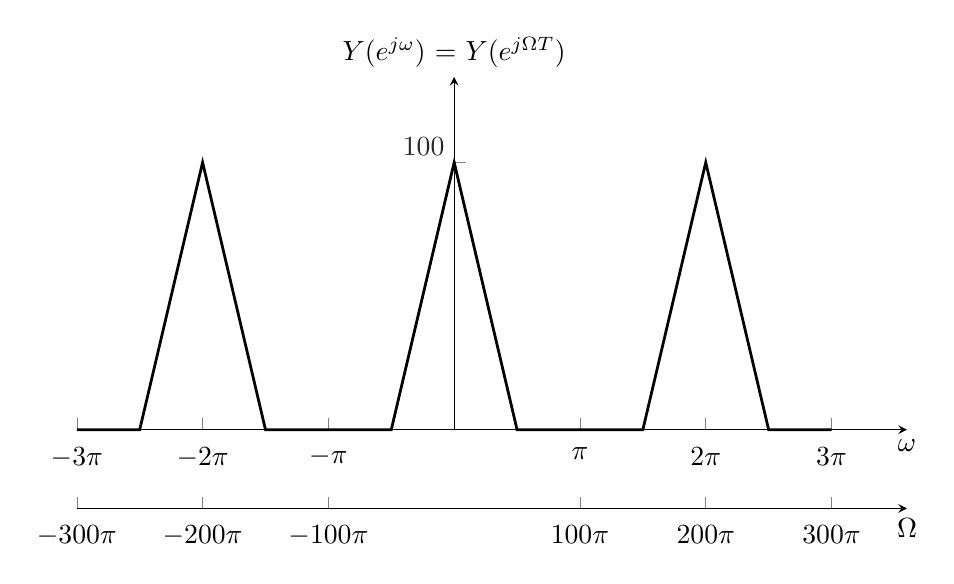
\begin{tikzpicture} 
\begin{axis}[
axis lines*=middle,
enlargelimits = upper, clip=false,
width=\textwidth,
height=0.5\textwidth,
ymin=0,
ymax=1.2,
xmin=-30,
xmax=30,
axis line style={->,>=stealth},
xlabel={$\omega$},
ylabel={$Y(e^{j\omega})$ = $Y(e^{j\Omega T})$},
yticklabel style = {yshift=0.2cm},
xticklabel style = {yshift=-0.1cm},
every axis x label/.style={
	at={(ticklabel* cs:1)},
	anchor=north,
},
every axis y label/.style={
	at={(ticklabel* cs:1)},
	anchor=south,
},
ytick=1,
yticklabels={$100$},
xtick={-30, -20, -10,  10, 20, 30},
xticklabels={$-3\pi$, $-2\pi$, $-\pi$, $\pi$, $2\pi$, $3\pi$},
every outer y axis line/.append style={white!15!black},
every y tick label/.append style={font=\color{white!15!black}},
legend style={draw=white!15!black,fill=white,legend cell align=left}]
%\addplot[black, line width=1.5pt] coordinates {(-30, 1) (30, 1)};
\addplot[black, line width=1pt, domain=-30:30, samples=101] coordinates {(-30, 0) (-25, 0) (-20, 1) (-15, 0) (-5, 0) (0, 1) (5, 0) (15, 0) (20, 1) (25, 0) (30, 0)};
\end{axis}

% extra x axis
\begin{axis}[yshift=-1cm,
axis lines*=middle,
enlargelimits = upper, clip=false,
xmin=-30,
xmax=30,
width=\textwidth,
height=0.5\textwidth,
hide y axis,
axis line style={->,>=stealth},
xlabel={$\Omega$},
xticklabel style = {yshift=-0.1cm},
every axis x label/.style={
	at={(ticklabel* cs:1)},
	anchor=north,
},
xtick={-30, -20, -10,  10, 20, 30},
xticklabels={$-300\pi$, $-200\pi$, $-100\pi$, $100\pi$, $200\pi$, $300\pi$},
every outer y axis line/.append style={white!15!black},
every y tick label/.append style={font=\color{white!15!black}},
legend style={draw=white!15!black,fill=white,legend cell align=left}]
\addplot[draw=none] {1};
\end{axis}

\end{tikzpicture}}
		\caption{Scenario 1: $\Omega_s = 200\pi$}
	\end{subfigure}%
	~ %add desired spacing between images, e. g. ~, \quad, \qquad etc.
	%(or a blank line to force the subfigure onto a new line)
	\begin{subfigure}[h!]{0.5\textwidth}
		\resizebox{\textwidth}{!}{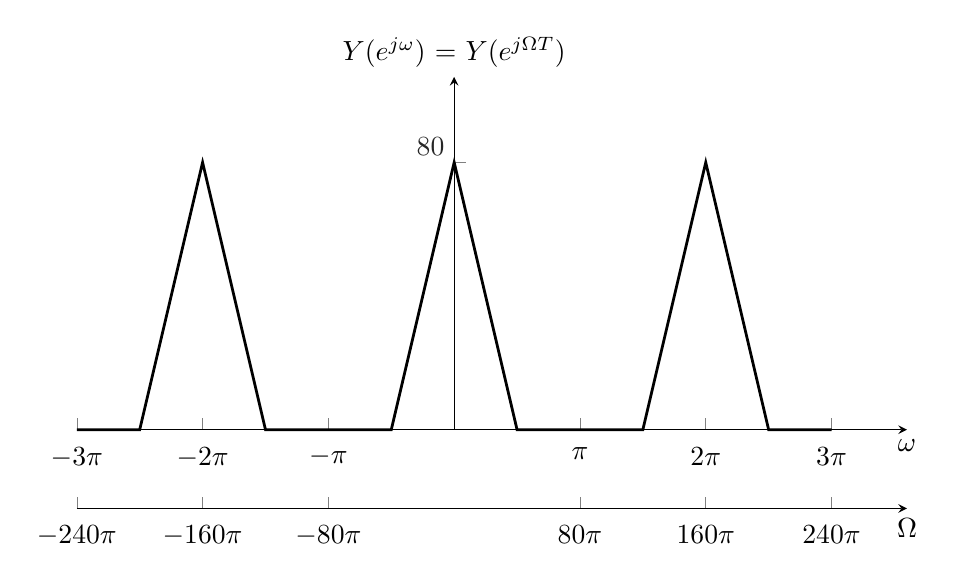
\begin{tikzpicture} 
\begin{axis}[
axis lines*=middle,
enlargelimits = upper, clip=false,
width=\textwidth,
height=0.5\textwidth,
ymin=0,
ymax=1.2,
xmin=-30,
xmax=30,
axis line style={->,>=stealth},
xlabel={$\omega$},
ylabel={$Y(e^{j\omega})$ = $Y(e^{j\Omega T})$},
yticklabel style = {yshift=0.2cm},
xticklabel style = {yshift=-0.1cm},
every axis x label/.style={
	at={(ticklabel* cs:1)},
	anchor=north,
},
every axis y label/.style={
	at={(ticklabel* cs:1)},
	anchor=south,
},
ytick=1,
yticklabels={$80$},
xtick={-30, -20, -10,  10, 20, 30},
xticklabels={$-3\pi$, $-2\pi$, $-\pi$, $\pi$, $2\pi$, $3\pi$},
every outer y axis line/.append style={white!15!black},
every y tick label/.append style={font=\color{white!15!black}},
legend style={draw=white!15!black,fill=white,legend cell align=left}]
%\addplot[black, line width=1.5pt] coordinates {(-30, 1) (30, 1)};
\addplot[black, line width=1pt, domain=-30:30, samples=101] coordinates {(-30, 0) (-25, 0) (-20, 1) (-15, 0) (-5, 0) (0, 1) (5, 0) (15, 0) (20, 1) (25, 0) (30, 0)};
\end{axis}

% extra x axis
\begin{axis}[yshift=-1cm,
axis lines*=middle,
enlargelimits = upper, clip=false,
xmin=-30,
xmax=30,
width=\textwidth,
height=0.5\textwidth,
hide y axis,
axis line style={->,>=stealth},
xlabel={$\Omega$},
xticklabel style = {yshift=-0.1cm},
every axis x label/.style={
	at={(ticklabel* cs:1)},
	anchor=north,
},
xtick={-30, -20, -10,  10, 20, 30},
xticklabels={$-240\pi$, $-160\pi$, $-80\pi$, $80\pi$, $160\pi$, $240\pi$},
every outer y axis line/.append style={white!15!black},
every y tick label/.append style={font=\color{white!15!black}},
legend style={draw=white!15!black,fill=white,legend cell align=left}]
\addplot[draw=none] {1};
\end{axis}

\end{tikzpicture}}
		\caption{Scenario 2: $\Omega_s = 160\pi$}
	\end{subfigure}
	\caption{Output spectrum obtained at the output of the discrete-time LTI system when (a) $\Omega_s = 200\pi$ and (b) $\Omega_s = 160\pi$.}
\end{figure}
	
Note that, expect for a scaling factor, the two spectra are the same when compared with respect to the normalized frequency $\omega$. That is, both of them have maximum frequency $\pi/2$. On the other hand, when compared with respect to the actual frequency $\Omega$, the spectra differ. Specifically, in the first scenario the output spectrum has maximum frequency $50\pi$, whereas in the second scenario the output spectrum has maximum frequency $40\pi$.
	
\subsection{(c)}
After reconstruction with the ideal lowpass filter with cutoff frequency $\Omega_s/2$:

\begin{figure}[h!]
	\centering
	\begin{subfigure}[h!]{0.5\textwidth}
		\resizebox{\textwidth}{!}{\def\fs{20}
\begin{tikzpicture} 
\begin{axis}[
axis lines*=middle,
enlargelimits = upper, clip=false,
width=\textwidth,
height=0.5\textwidth,
ymin=0,
ymax=1.2,
xmin=-30,
xmax=30,
axis line style={->,>=stealth},
xlabel={$\Omega$},
ylabel={$Y_r(j\Omega)$},
yticklabel style = {yshift=0.2cm},
xticklabel style = {yshift=-0.1cm},
every axis x label/.style={
	at={(ticklabel* cs:1)},
	anchor=north,
},
every axis y label/.style={
	at={(ticklabel* cs:1)},
	anchor=south,
},
ytick=1,
yticklabels={$1$},
xtick={-5, 5},
xticklabels={$-50\pi$, $50\pi$},
every outer y axis line/.append style={white!15!black},
every y tick label/.append style={font=\color{white!15!black}},
legend style={draw=white!15!black,fill=white,legend cell align=left}]
%\addplot[black, line width=1.5pt] coordinates {(-30, 1) (30, 1)};
\addplot[black, line width=1pt, domain=-30:30, samples=101] coordinates {(-30, 0) (-5, 0) (0, 1) (5, 0) (30, 0)};
\end{axis}

\end{tikzpicture}}
		\caption{Scenario 1: $\Omega_s = 200\pi$}
	\end{subfigure}%
	~ %add desired spacing between images, e. g. ~, \quad, \qquad etc.
	%(or a blank line to force the subfigure onto a new line)
	\begin{subfigure}[h!]{0.5\textwidth}
		\resizebox{\textwidth}{!}{\def\fs{20}
\begin{tikzpicture} 
\begin{axis}[
axis lines*=middle,
enlargelimits = upper, clip=false,
width=\textwidth,
height=0.5\textwidth,
ymin=0,
ymax=1.2,
xmin=-30,
xmax=30,
axis line style={->,>=stealth},
xlabel={$\Omega$},
ylabel={$Y_r(j\Omega)$},
yticklabel style = {yshift=0.2cm},
xticklabel style = {yshift=-0.1cm},
every axis x label/.style={
	at={(ticklabel* cs:1)},
	anchor=north,
},
every axis y label/.style={
	at={(ticklabel* cs:1)},
	anchor=south,
},
ytick=1,
yticklabels={$1$},
xtick={-4, 4},
xticklabels={$-40\pi$, $40\pi$},
every outer y axis line/.append style={white!15!black},
every y tick label/.append style={font=\color{white!15!black}},
legend style={draw=white!15!black,fill=white,legend cell align=left}]
%\addplot[black, line width=1.5pt] coordinates {(-30, 1) (30, 1)};
\addplot[black, line width=1pt, domain=-30:30, samples=101] coordinates {(-30, 0) (-4, 0) (0, 1) (4, 0) (30, 0)};
\end{axis}

\end{tikzpicture}}
		\caption{Scenario 2: $\Omega_s = 160\pi$}
	\end{subfigure}
	\caption{Output spectrum after reconstruction when (a) $\Omega_s = 200\pi$ and (b) $\Omega_s = 160\pi$.}
\end{figure}
	
Both spectra have amplitude 1, since, by definition, the ideal lowpass filter has gain $T$ at frequency zero.	
	
Note that even though the DSP operation was the same in both scenarios, the result in continuous time was different. This problem illustrates that the outcome depends on the sampling frequency.
	
\section{Problem 2}
\subsection{(a)}
To obtain a white noise spectrum after sampling, the sampling period $T$ must be such that the linear taper part of the spectrum replicas perfectly overlaps as illustrated in the figure below:

\begin{figure}[h!]
	\centering
	\resizebox{0.8\textwidth}{!}{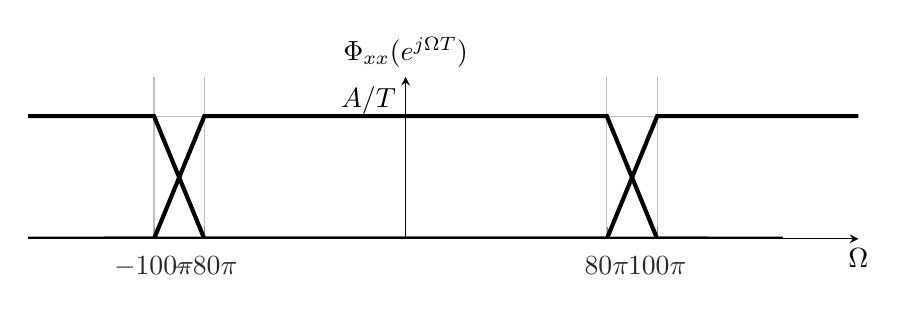
\begin{tikzpicture} 
\begin{axis}[
axis lines*=middle,
enlargelimits = upper, clip=true,
width=\textwidth,
height=0.3\textwidth,
ymin=0,
ymax=1.2,
xmin=-15,
xmax=15,
axis line style={->,>=stealth},
xlabel={$\Omega$},
ylabel={$\Phi_{xx}(e^{j\Omega T})$},
yticklabel style = {yshift=0.2cm},
xticklabel style = {yshift=-0.1cm},
every axis x label/.style={
	at={(ticklabel* cs:1)},
	anchor=north,
},
every axis y label/.style={
	at={(ticklabel* cs:1)},
	anchor=south,
},
ytick=1,
yticklabels={$A/T$},
xtick={-10,  10},
xticklabels={$-100\pi$, $100\pi$},
extra x ticks={-8, 8}, extra x tick labels={ $-80\pi$,  $80\pi$},
extra tick style={grid=major},
every outer y axis line/.append style={white!15!black},
every x tick label/.append style={font=\color{white!15!black}},
grid=major,
legend style={draw=white!15!black,fill=white,legend cell align=left}]

\addplot[black, line width=1.5pt] coordinates {(-15, 0) (-10, 0) (-8, 1) (8, 1) (10, 0) (15, 0)};
\addplot[black, line width=1.5pt] coordinates {(-12, 0) (-10+18, 0) (-8+18, 1) (8+18, 1) (10+18, 0) (15+18, 0)} node[->, pos=0.8, black, pin={[pin edge={black, thick}]30:{Linear taper}}, inner sep=0pt] {};
\addplot[black, line width=1.5pt] coordinates {(-15-18, 0) (-10-18, 0) (-8-18, 1) (8-18, 1) (10-18, 0) (12, 0)};
\end{axis}
\end{tikzpicture}}
	\caption{Output spectrum after reconstruction when (a) $\Omega_s = 200\pi$ and (b) $\Omega_s = 160\pi$.}
	\label{fig:linear_taper}
\end{figure}

This occurs when $\Omega_s = 180\pi = 2\pi/T$. Therefore, $T = 1/90$.

\subsection{(b)}

From Figure~\ref{fig:linear_taper}, we clearly see that
\begin{equation}
\sigma_x^2 = \frac{A}{T} = 90A
\end{equation}

\subsection{(c)}

To obtain a white discrete-time PSD, we must have
\begin{equation}
\Phi_{xx}(e^{j\omega}) =\sigma_x^2, ~\text{for any}~\omega
\end{equation}

We can write an equivalent condition for the autocorrelation function by calculating the inverse Fourier transform:
\begin{equation}
\phi_{xx}[m] = \sigma_x^2\delta[m] = \begin{cases}
\sigma_x^2, & m = 0 \\
0, & \text{otherwise}
\end{cases}
\end{equation}

Since the discrete-time autocorrelation function is simply the sampled continuous-time autocorrelation function ($\phi_{xx}[m] = \phi_{x_cx_c}(mT)$), it follows that

\begin{equation}
\phi_{x_cx_c}(mT) = \sigma_x^2\delta[m] = \begin{cases}
\sigma_x^2, & m = 0 \\
0, & \text{otherwise}
\end{cases}
\end{equation}

Therefore, we can only obtain a discrete-time white noise from a non-white continuous-time noise if the continuous-time autocorrelation function is zero at the sampling instants $\tau = mT$, except at $\tau = mT = 0$.

\section{Problem 3}	
\subsection{(a)}

Recall the following Fourier transform pairs:
\begin{align}
a(t) = c &\Longleftrightarrow A(j\Omega) = 2\pi\delta(\Omega) \tag{constant} \\
a(t) = b\cos(\Omega_0t - \phi) &\Longleftrightarrow A(j\Omega) = b\pi(\delta(\Omega-\Omega_0)e^{-j\phi} + \delta(\Omega+\Omega_0)e^{j\phi}) \tag{cosine}
\end{align}

Now we can write an equation for $X_c(j\Omega)$,
\begin{equation}
X_c(j\Omega) = 30\pi\delta(\Omega) + 10\pi(\delta(\Omega-600\pi) + \delta(\Omega+600\pi)) + 5\pi(\delta(\Omega-1500\pi)e^{-j\pi/3} + \delta(\Omega+1500\pi)e^{j\pi/3})
\end{equation}

\begin{center}
	\resizebox{0.5\linewidth}{!}{
		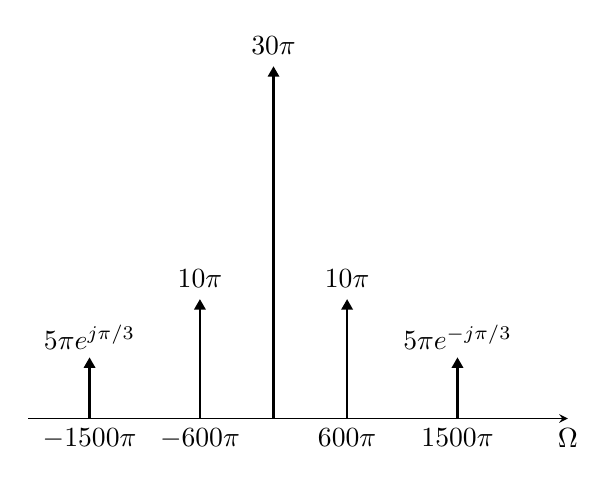
\begin{tikzpicture} 
		\begin{axis}[
		axis lines*=middle,
		enlargelimits = upper,
		xmax=2000,
		xmin=-2000,
		ymin=0,
		ymax=35,
		hide y axis,
		axis line style={->,>=stealth},
		ylabel={$X_c(j\Omega)$},
		xlabel={$\Omega$},
		every axis x label/.style={
			at={(ticklabel* cs:1)},
			anchor=north,
		},
		every axis y label/.style={
			at={(ticklabel* cs:1)},
			anchor=south,
		},
		xtick={-1500, -600, 0, 600, 1500},
		xticklabels={$-1500\pi$, $-600\pi$, $0$, $600\pi$, $1500\pi$},
		xticklabel style = {xshift=0cm},
		every outer y axis line/.append style={white!15!black},
		every y tick label/.append style={font=\color{white!15!black}},
		legend style={draw=white!15!black,fill=white,legend cell align=left}]
		\addplot[dirac, mark=triangle*, fill=black, mark options={scale=0.75, fill=black}, line width=1pt] coordinates {(-1500, 5) (-600, 10) (0, 30) (600, 10) (1500, 5)};
		\node at (axis cs: -1500, 7) {$5\pi e^{j\pi/3}$};
		\node at (axis cs: 1500, 7) {$5\pi e^{-j\pi/3}$};
		\node at (axis cs: -600, 12) {$10\pi$};
		\node at (axis cs: 600, 12) {$10\pi$};
		\node at (axis cs: 0, 32) {$30\pi$};
		\end{axis}
		\end{tikzpicture}
}
\end{center}

\subsection{(b)}

After sampling, there'll be replicas of the spectrum at multiples of $\Omega_s = 2\pi/T = 4000\pi$. Since the original signal is band-limited with highest frequency is $1500\pi < \Omega_s/2$, there will not be spectrum overlapping and aliasing distortion:

\begin{center}
	\resizebox{\linewidth}{!}{
		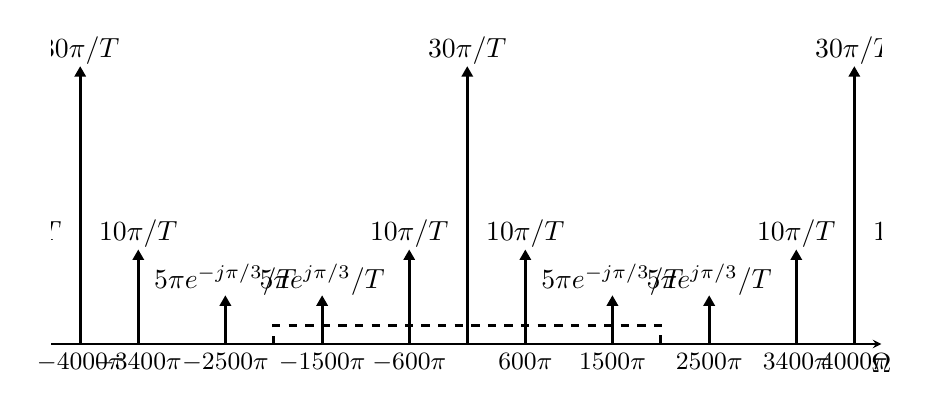
\begin{tikzpicture} 
		\begin{axis}[
		axis lines*=middle,
		enlargelimits = upper,clip=true,
		xmax=3500,
		xmin=-4300,
		ymin=0,
		ymax=35,
		hide y axis,
		width=\textwidth,
		height=0.5\textwidth,
		axis line style={->,>=stealth},
		ylabel={$X_c(j\Omega)$},
		xlabel={$\Omega$},
		every axis x label/.style={
			at={(ticklabel* cs:1)},
			anchor=north,
		},
		every axis y label/.style={
			at={(ticklabel* cs:1)},
			anchor=south,
		},
		xtick={-4000, -3400, -2500, -1500, -600, 0, 600, 1500, 2500, 3400, 4000},
		xticklabels={\small $-4000\pi$, \small $-3400\pi$, \small $-2500\pi$, \small $-1500\pi$, \small$-600\pi$, \small $0$, \small $600\pi$, \small $1500\pi$, \small $2500\pi$, \small $3400\pi$, \small $4000\pi$},
		xticklabel style = {xshift=0cm},
		every outer y axis line/.append style={white!15!black},
		every y tick label/.append style={font=\color{white!15!black}},
		legend style={draw=white!15!black,fill=white,legend cell align=left}]
		\addplot[dirac, mark=triangle*, fill=black, mark options={scale=0.75, fill=black}, line width=1pt] coordinates {(-1500, 5) (-600, 10) (0, 30) (600, 10) (1500, 5)};
		\node at (axis cs: -1500, 7) {$5\pi e^{j\pi/3}/T$};
		\node at (axis cs: 1500, 7) {$5\pi e^{-j\pi/3}/T$};
		\node at (axis cs: -600, 12) {$10\pi/T$};
		\node at (axis cs: 600, 12) {$10\pi/T$};
		\node at (axis cs: 0, 32) {$30\pi/T$};
		
		\addplot[dirac, mark=triangle*, fill=black, mark options={scale=0.75, fill=black}, line width=1pt] coordinates {(-1500-4000, 5) (-600-4000, 10) (0-4000, 30) (600-4000, 10) (1500-4000, 5)};
		\node at (axis cs: -1500-4000, 7) {$5\pi e^{j\pi/3}/T$};
		\node at (axis cs: 1500-4000, 7) {$5\pi e^{-j\pi/3}/T$};
		\node at (axis cs: -600-4000, 12) {$10\pi/T$};
		\node at (axis cs: 600-4000, 12) {$10\pi/T$};
		\node at (axis cs: 0-4000, 32) {$30\pi/T$};
		
		
		\addplot[dirac, mark=triangle*, fill=black, mark options={scale=0.75, fill=black}, line width=1pt] coordinates {(-1500+4000, 5) (-600+4000, 10) (0+4000, 30) (600+4000, 10) (1500+4000, 5)};
		\node at (axis cs: -1500+4000, 7) {$5\pi e^{j\pi/3}/T$};
		\node at (axis cs: 1500+4000, 7) {$5\pi e^{-j\pi/3}/T$};
		\node at (axis cs: -600+4000, 12) {$10\pi/T$};
		\node at (axis cs: 600+4000, 12) {$10\pi/T$};
		\node at (axis cs: 0+4000, 32) {$30\pi/T$};
		
		\addplot[dashed, line width=1pt] coordinates {(-2000, 0) (-2000, 2) (2000, 2) (2000, 0)};
		\end{axis}
		\end{tikzpicture}
	}
\end{center}

The reconstruction filter is indicated by the dashed line in the figure above.

The reconstructed signal is given by

\begin{equation}
X_r(j\Omega) = 30\pi\delta(\Omega) + 10\pi(\delta(\Omega-600\pi) + \delta(\Omega+600\pi)) + 5\pi(\delta(\Omega-1500\pi)e^{-j\pi/3} + \delta(\Omega+1500\pi)e^{j\pi/3})
\end{equation}

\noindent and in the time domain:
\begin{equation}
X_r(t) = 15 + 10\cos(600\pi t) + 5\cos(1500\pi t - \pi/3) = x_c(t) \tag{exactly equal to the original signal}
\end{equation}

\subsection{(c)}

By choosing $T = 1/750$, we obtain the following spectrum. Note that the components of the term $5\cos(1500\pi t-\pi/3)$ now fall on the origin. 


\begin{center}
	\resizebox{\linewidth}{!}{
		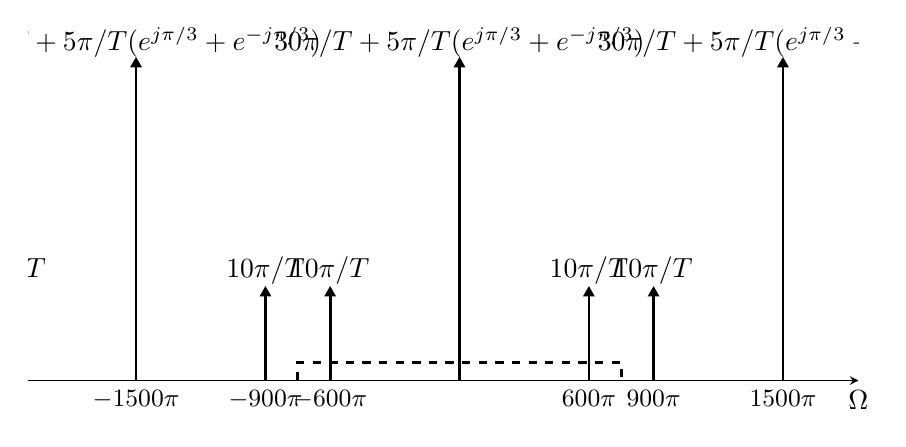
\begin{tikzpicture} 
		\begin{axis}[
		axis lines*=middle,
		enlargelimits = upper,clip=true,
		xmax=1500,
		xmin=-2000,
		ymin=0,
		ymax=35,
		hide y axis,
		width=\textwidth,
		height=0.5\textwidth,
		axis line style={->,>=stealth},
		ylabel={$X_c(j\Omega)$},
		xlabel={$\Omega$},
		every axis x label/.style={
			at={(ticklabel* cs:1)},
			anchor=north,
		},
		every axis y label/.style={
			at={(ticklabel* cs:1)},
			anchor=south,
		},
		xtick={-1500, -900, -600, 0, 600, 900, 1500},
		xticklabels={\small $-1500\pi$, \small $-900\pi$, \small $-600\pi$, \small $0$, \small $600\pi$, \small $900\pi$, \small $1500\pi$},
		xticklabel style = {xshift=0cm},
		every outer y axis line/.append style={white!15!black},
		every y tick label/.append style={font=\color{white!15!black}},
		legend style={draw=white!15!black,fill=white,legend cell align=left}]
		\addplot[dirac, mark=triangle*, fill=black, mark options={scale=0.75, fill=black}, line width=1pt] coordinates {(-600, 10) (0, 35) (600, 10)};
		\node at (axis cs: -600, 12) {$10\pi/T$};
		\node at (axis cs: 600, 12) {$10\pi/T$};
		\node at (axis cs: 0, 37) {$30\pi/T + 5\pi/T(e^{j\pi/3}+e^{-j\pi/3})$};
		
		\addplot[dirac, mark=triangle*, fill=black, mark options={scale=0.75, fill=black}, line width=1pt] coordinates {(-600-1500, 10) (0-1500, 35) (600-1500, 10)};
		\node at (axis cs: -600-1500, 12) {$10\pi/T$};
		\node at (axis cs: 600-1500, 12) {$10\pi/T$};
		\node at (axis cs: 0-1500, 37) {$30\pi/T + 5\pi/T(e^{j\pi/3}+e^{-j\pi/3})$};
		
		
		\addplot[dirac, mark=triangle*, fill=black, mark options={scale=0.75, fill=black}, line width=1pt] coordinates { (-600+1500, 10) (0+1500, 35) (600+1500, 10)};
		\node at (axis cs: -600+1500, 12) {$10\pi/T$};
		\node at (axis cs: 600+1500, 12) {$10\pi/T$};
		\node at (axis cs: 0+1500, 37) {$30\pi/T + 5\pi/T(e^{j\pi/3}+e^{-j\pi/3})$};
		
		\addplot[dashed, line width=1pt] coordinates {(-750, 0) (-750, 2) (750, 2) (750, 0)};
		\end{axis}
		\end{tikzpicture}
	}
\end{center}

After the reconstruction filter depicted in the image above by the dashed lines, we obtain:

\begin{align} \nonumber
X_r(j\Omega) &= (30\pi + 5\pi(e^{j\pi/3}+e^{-j\pi/3}))\delta(\Omega) + 10\pi(\delta(\Omega-600\pi) + \delta(\Omega+600\pi)) \\ \nonumber
&= (30\pi + 10\pi\cos(\pi/3))\delta(\Omega) + 10\pi(\delta(\Omega-600\pi) + \delta(\Omega+600\pi)) \\
&= 35\pi\delta(\Omega) + 10\pi(\delta(\Omega-600\pi) + \delta(\Omega+600\pi))
\end{align}

\noindent and in time domain:
\begin{equation}
X_r(t) = 35/2 + 10\cos(600\pi t)
\end{equation}
	
\section{Problem 4}
\subsection{(a)}

The maximum value of $t_d$ will occur when the sound source is along the dashed line and above the first (top) microphone. This way, the sound will reach microphone 1, and only after propagating the distance $d$, it will reach the second microphone. Similarly, the minimum negative value of $t_d$ will occur when the sound source is along the dashed line, but now below the second microphone. Therefore,

\begin{equation}
-\frac{d}{c} \leq t_d \leq \frac{d}{c}
\end{equation}

\subsection{(b)}

\begin{align} \nonumber
\phi_{x_1x_2}[m] &= \E\{x_1[n+m]x_2[n]\} \\ \nonumber
&=\E\{(\alpha_1 s[n+m]+v_1[n+m])(\alpha_2 s_D[n]+v_{2}[n])\} \\ \nonumber
&=\E\{(\alpha_1 s[n+m]+v_1[n+m])(\alpha_2 s[n+D]+v_{2}[n])\} \\
&= \alpha_1\alpha_2\E(s[n+m]s[n+D]) + \alpha_1\E(s[n+m]v_2[n]) + \alpha_2\E(s[n+D]v_1[n+m]) + \E(v_2[n]v_1[n+m])
\end{align}

From the assumption that the signal and noises are all statistically independent, the last three terms are zero. Therefore, 
\begin{align} \nonumber
\phi_{x_1x_2}[m] &= \alpha_1\alpha_2\E(s[n+m]s[n+D]) \\
&= \alpha_1\alpha_2\phi_{ss}[m-D]
\end{align}

\subsection{(c)}
\begin{align} \nonumber
\Phi_{x_1x_2}(e^{j\omega}) &= \mathcal{F}\{\phi_{x_1x_2}[m]\} = \alpha_1\alpha_2\mathcal{F}\{\phi_{ss}[m-D]\} \\
&= \alpha_1\alpha_2\Phi_{ss}(e^{j\omega})e^{-j\omega D},
\end{align}
\noindent where the last equality follows from the time-delay property of the DTFT.


\subsection{(d)}

From part (b) $\phi_{x_1x_2}[m] = \alpha_1\alpha_2\phi_{ss}[m-D]$. Since $\phi_{ss}[n]$ is an autocorrelation function, its maximum value occurs when $n = 0$. Therefore, the maximum value of $\phi_{x_1x_2}[m]$ will occur when $m = D$.

In an algorithm implementation, we can estimate $\phi_{x_1x_2}[m]$ from measurement, and find for which value of $m$, $\phi_{x_1x_2}[m]$ is maximized:

\begin{equation}
m^\star = \mathrm{argmax}\phi_{x_1x_2}[m].
\end{equation}

Then, we can finally estimate $t_d = m^\star T$.

\subsection{(e)}

Using the result from part (c): 
\begin{equation}
\Phi_{x_1x_2}(e^{j\omega}) = \alpha_1\alpha_2\Phi_{ss}(e^{j\omega})e^{-j\omega D} = \alpha_1\alpha_2\sigma_s^2e^{-j\omega D}
\end{equation}

We can calculate the cross-correlation function by simply taking the inverse DTFT of $\Phi_{x_1x_2}(e^{j\omega})$:

\begin{align} \nonumber
\phi_{x_1x_2}[m] &= \int_{-\pi}^{\pi}\Phi_{x_1x_2}(e^{j\omega})e^{j\omega m}d\omega \\
&=\alpha_1\alpha_2\sigma_s^2\int_{-\pi}^{\pi}e^{-j\omega D}e^{j\omega m} d\omega \\ 
&=\alpha_1\alpha_2\sigma_s^2\int_{-\pi}^{\pi}e^{j\omega(m-D)} d\omega \\ 
&=\alpha_1\alpha_2\sigma_s^2\bigg[\frac{1}{j(m-D)}e^{j\omega(m-D)}\bigg]_{-\pi}^{\pi} \\
&=\alpha_1\alpha_2\sigma_s^2\frac{\sin(\pi(m-D))}{\pi(m-D)} \\  
&=\alpha_1\alpha_2\sigma_s^2\mathrm{sinc}(m-D)
\end{align}

If $D$ is an integer, then $\mathrm{sinc}(m-D)$ is only non-zero when $m = D$. Therefore, we can write:
\begin{align} \nonumber
\phi_{x_1x_2}[m] = \begin{cases}
\alpha_1\alpha_2\sigma_s^2\delta[m-D], & \text{when $D$ is integer} \\
\alpha_1\alpha_2\sigma_s^2\mathrm{sinc}(m-D), & \text{otherwise}
\end{cases}
\end{align}
\end{document}